\chapter{Ausganglage} % (fold)
\label{cha:Ausganglage}

\section{Geschichtlicher Hintergrund} % (fold)
\label{sec:Geschichtlicher Hintergrund}

Die Firma Komm.One existiert in ihrer heutigen Form erst seit Mitte 2018. Die zunächst unter dem Namen ITEOS zusammengeschlossenen Zweckverbände KDRS, KIRU, und KIVBF mitsamt der Datenzentrale Baden-Württemberg, gegründete Anstalt öffentlichen Rechts wird vom Land Baden-Württemberg und den Kommunen im Land gemeinsam getragen. Die in 1969 beginnenden Gründungen von kommunalen Rechenzentren in Ulm, Heidelberg, Freiburg, Stuttgart, Heilbronn, Reutlingen, Karlsruhe und der Datenzentrale führt nach und nach zur Entstehung der Zweckverbände. Der erste Zweckverband bildet sich im Jahr 1995, als das Rechenzentrum Mittlerer Neckar zum Zweckverband Kommunale Datenverarbeitung Region Stuttgart (KDRS) wird. Im Jahr 2002 schließen sich die Rechenzentren Reutlingen und Ulm zum Zweckverband Kommunale Informationsverarbeitung Reutlingen-Ulm (KIRU) zusammen. Zu guter Letzt schließen sich 2003 die Standorte Karlsruhe, Freiburg, Heidelberg und Heilbronn zum Zweckverband Kommunale Informationsverarbeitung Baden-Franken (KIVBF) zusammen. \footcite[Vgl.][auch im Folgenden]{o.V..2022}

Auf Grund der Entstehung der Komm.One aus mehreren einzelnen Standorten, die sich erst über die Jahre zusammengeschlossen haben und lange Zeit vollständig unabhängig voneinander waren und der noch sehr frischen Zusammenschließung gibt es intern immer noch große Unterschiede zwischen Standorten. Angefangen bei Benutzernamen der Mitarbeiter bis hin zu Servern hat in vielen Bereichen noch jeder Standort seine eigenen Tücken. Die Harmonisierung dieser kleinen und großen Unterschiede ist seit Beginn des Zusammenschlusses ein großes Thema in der Firma, das allerdings nicht von jetzt auf gleich, sondern nach und nach umgesetzt werden muss. Bereits im Jahr 2019 wurde die interne WLAN Infrastruktur komplett überarbeitet im Zuge eines Redesigns des gesamten Campusnetzwerkes.

An diesen Schritt anknüpfend steht nun die Harmonisierung von VPN-Einzelplatz-Lösungen bevor.

% section Geschichtlicher HintergrundGeschichtlicher Hintergrund (end)

\section{VPN-Situation intern} % (fold)
\label{sec:VPN-Situation intern}

Aktuell werden drei verschiedene VPN-Lösungen intern verwendet. Dazu gehören Checkpoint-VPN, NCP-VPN und Anyconnect-VPN. Checkpoint wurde von dem Zweckverband KIRU verwendet, also in den östlichen Standorten von Baden-Württemberg. NCP findet im westlichen Teil des Landes, vom Zweckverband KIVBF, die meiste Verwendung. Die Datenzentrale verwendet vorzugsweise Anyconnect. Zu diesem Zeitpunkt sind 894 Clients in Checkpoint-VPN registriert, wovon 889 interne Mitarbeiter und die Übrigen Testclients sind. In der Datenzentrale sind 317 Anyconnect-Zugänge im Betrieb. Bei den NCP-VPN Clients wird aktuell nicht zwischen internen Mitarbeitern und externen Dienstleistern unterschieden. Das muss aus Sicherheitsgründen geändert werden. Mitarbeiter haben eine andere Sicherheitsstufe als externe Dienstleister, die keinen Zugang zu internen Systemen haben dürfen. Hier sind 1195 Clients in Betrieb, wovon 856 von Mitarbeitern der Komm.One verwendet werden und 68 von der Tochterfirma Endica. Die restlichen 271 gehören zu den externen Dienstleistern. 

NCP läuft auf zwölf virtuellen Maschinen, die in Karlsruhe stehen. Davon sind zwei Managementserver und zehn Gateways. Je Gateway können 250 aktive Verbindungen hergestellt werden. Allerdings ist hier zu beachten, dass jeweils zwei Gateways redundant agieren und somit jeweils zwei Gateways 250 aktive Verbindungen erlauben. Angesicht der 1195 Clients ist der aktuelle Aufbau also auf bis zu 1250 aktive Verbindungen ausgelegt. Das bedeutet das System hat noch eine ganze Menge an möglichen Verbindungen frei. \footcite[Vgl.][auch im Folgenden]{Beier.2022a}

\begin{figure}[htb]
  \centering
  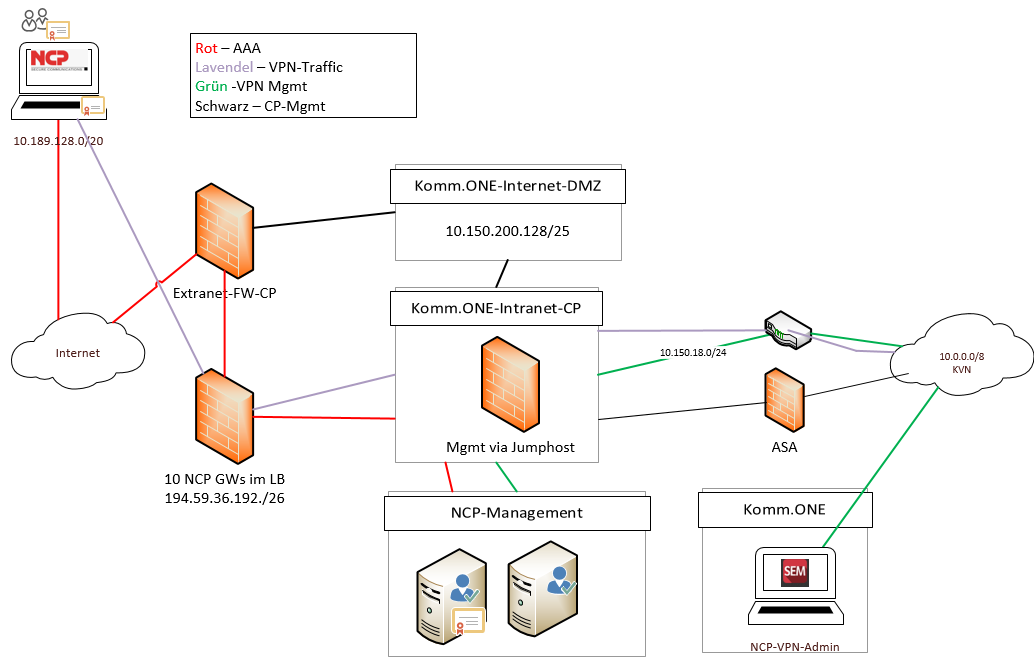
\includegraphics[width=14cm]{graphics/NCP.png}
  \caption[Logischer Aufbau der Service Architektur von VPN-Einzelplatz-NCP]{Logischer Aufbau der Service Architektur von VPN-Einzelplatz-NCP \footnotemark}
  \label{abb:NCPAufbau}
\end{figure}
\footnotetext{Entnommen aus: \cite{Beier.2022a}}

Abbildung \ref{abb:NCPAufbau} zeigt den logischen Aufbau der Service Architektur des VPN-Einzelplatz-NCP. Hierbei zeigen die roten Linien den Verbindungsaufbau bei der Anmeldung und die lavendelfarbenen Linien den Verlauf des VPN-Tunnels. Die grünen und schwarzen Linien zeigen lediglich Verbindungen zur Administrierung. Gut in der Grafik zu erkennen ist die Authentifizierung, die hier im NCP-Management stattfindet und das Zertifikat mit dem Passwort und Gerät abgleicht.

Für die Bereitstellung der Anyconnect-VPN-Struktur sind zwei virtuelle Maschinen und ein Hardwareserver im Betrieb. Diese stehen am Standort Stuttgart. \footcite[Vgl.][auch im Folgenden]{Beier.2022b}

\begin{figure}[htb]
  \centering
  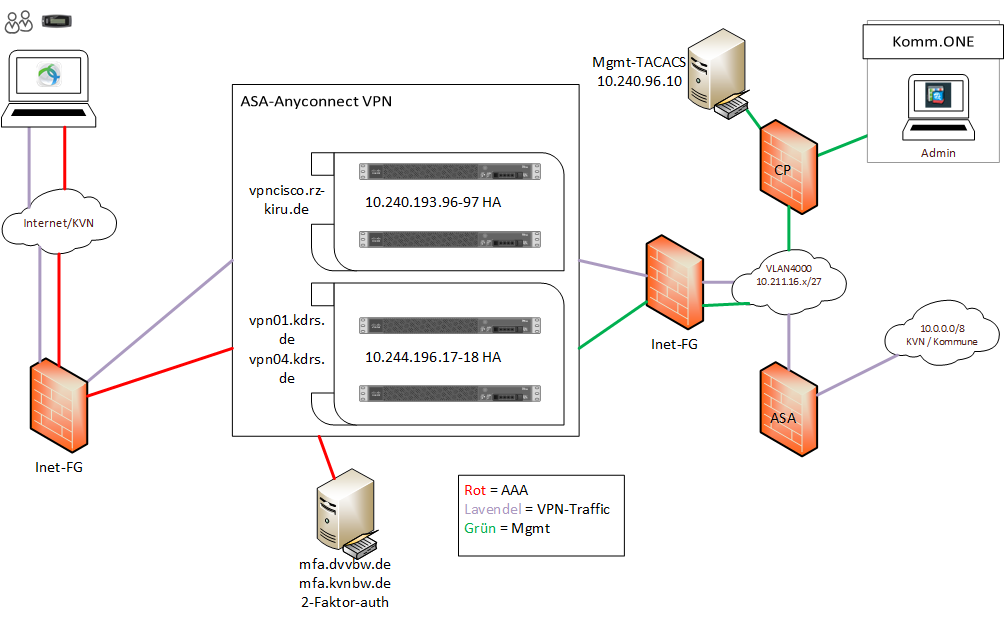
\includegraphics[width=14cm]{graphics/Anyconnect.png}
  \caption[Logischer Aufbau der Service Architektur von Anyconnect-VPN]{Logischer Aufbau der Service Architektur von Anyconnect-VPN \footnotemark}
  \label{abb:AnyconnectAufbau}
\end{figure}
\footnotetext{Entnommen aus: \cite{Beier.2022b}}

Auch hier (Abb. \ref{abb:AnyconnectAufbau}) zeigen die roten Linien den Verbindungsverlauf der Anmeldung, die lavendelfarbenen Linien den Verlauf des VPN-Tunnels und die grünen Linien Administrationsverbindungen. Ebenso ist die Authentifizierung gut zu erkennen, welche über mfa.dvvbw.de und mfa.kvnbw.de erfolgt und durch einen Token und ein Passwort eine 2-Faktor-Authentifizierung schafft. 

\begin{figure}[htb]
  \centering
  
\includegraphics[width=14cm]{graphics/dhbw.png}
  \caption[Logischer Aufbau der Service Architektur von Checkpoint-VPN]{Logischer Aufbau der Service Architektur von Checkpoint-VPN}
  \label{abb:CheckpointAufbau}
\end{figure}

In Abbildung \ref{abb:CheckpointAufbau} wird die Service Architektur des internen Checkpoint-VPN Aufbaus dargestellt. In dieser Abbildung sind die einzelnen Verbindungen nicht farblich markiert. Bei der Anmeldung geht die Verbindung über die externe Firewall und den VPN Cluster zu mfa.komm.one. Hier findet, gleich wie bei der Anyconnect Lösung, die 2-Faktor-Authentifizierung mit Token und Passwort statt. Erst wenn diese abgeschlossen ist bekommt der Client Zugang zum Netzwerk der Komm.One.

% section VPN-Situation internVPN-Situation intern (end)

\section{Übersicht der unterschiedlichen Lösungen} % (fold)
\label{sec:Übersicht der unterschiedlichen Lösungen}

Der größte technische Unterschied zwischen den Lösungen besteht darin, dass bei NCP die Authentifizierung über ein Zertifikat und ein Passwort erfolgt, während bei Checkpoint und Anyconnect mit Tokens, hauptsächlich Softwaretokens, gearbeitet wird. 

NCP bietet mehrere Lizenzmodelle an. Das Modell namens „Perpetual“ bietet die Möglichkeit eine Lizenz zu aktuellen Bedingungen zu kaufen. In diesem Fall geht das Eigentum der Lizenz an den Kunden über. Beim „Pay-per-Use“-Modell von NCP erhält der Kunde alle benötigten Lizenzen in gewünschter Menge. Das schließt sowohl Client-, als auch Server und Management-Lizenzen ein. Die Kosten errechnen sich in diesem Modell nicht an den ausgegebenen Lizenzen, sondern an den tatsächlich verwendeten. Jeden Monat wird anhand eines monatlichen Reports die zu zahlende Rechnung bestimmt. Eine feste Rate für mindestens 5390 Lizenzen wird allerdings verlangt, auch wenn weniger Lizenzen im Monat benutzt wurden. Angesichts der Corona Pandemie bietet NCP ein Pandemie Angebot an. Dieses Angebot ist eine Mischung aus „Perpetual“ und „Pay-per-Use“. Der Kunde kauft eine feste Anzahl an Lizenzen, hat aber die Möglichkeit über mehr Lizenzen zu verfügen, wenn diese benötigt werden. Als viertes und letztes Modell bietet NCP die „Subscription“ an. In diesem Modell wird die Lizenz für einen im Vorfeld festgelegten Zeitraum erworben. In diesem Zeitraum stehen Updates kostenlos zur Verfügung. Nach Ablauf des Vertrages muss ein neuer geschlossen werden. Der Preis wird für den gesamten Zeitraum im Voraus bezahlt. \footnotemark
/\footnotetext{Vgl. \cite{o.V..2020} und \cite{Cisco.2022}}

Anyconnect und Checkpoint bieten nicht so viele Möglichkeiten. Hier müssen jeweils so viele Lizenzen erworben werden, wie potenzielle Lizenzen benötigt werden. Bei 1800 Mitarbeitern werden also 1800 Lizenzen benötigt, auch wenn nur 1500 Mitarbeiter in dem Jahr den VPN Zugang nutzen. Jede Lizenz ist jeweils für ein Jahr gültig. \footcite[Vgl.][]{CheckPointSoftware.2022}

% section Übersicht der unterschieden Lösungen (end)

% chapter (end)
